\documentclass[11pt,a4paper]{article}
\usepackage[utf8]{inputenc}
\usepackage{amsmath,amssymb,amsthm}
\usepackage[margin=1in]{geometry}
\usepackage{tikz}

\newtheorem{theorem}{Theorem}[section]
\newtheorem{proposition}[theorem]{Proposition}
\newtheorem{remark}[theorem]{Remark}

\title{Paper Z: Multi-Scale Entropic Stabilization, Discrete Flow Persistence, and Conceptual Synthesis of the Oasis Program}
\author{Mariano Panzano Caball\'e \\ Oasis Sovereign Architecture Research, Barcelona}
\date{November 2026}

\begin{document}
\maketitle

\begin{abstract}
Concluding the T--Z research sequence, Paper~Z synthesizes the numerical curvature probes on $\mathfrak{su}(3)$ and $L=2^4, 3^4$ lattices, the C99 Cabibbo--Marinari Wilson cross-benchmarks ($L=8^4, 12^4$), and a discrete inductive persistence theorem verified in pure Lean~4.36.0 (\texttt{PaperZ\_Sovereign\_Synthesis.lean}, \texttt{0 sorry}, \texttt{0 custom axioms}). We also present a six-stage pedagogical framework linking geometric stabilization, entropic compensation, and scale transitions. Explicitly, all theorems proved here establish conditional finite-step persistence under stated stabilization hypotheses and do not constitute an unconditional proof of 4D Yang--Mills existence or a mass gap on $\mathbb{R}^4$ or $\mathcal{S}'(\mathbb{R}^4)$.
\end{abstract}

\section{Six-Stage Conceptual Synthesis}
To make the geometric obstruction and its conditional stabilization accessible across disciplinary boundaries, the Oasis program organizes its workflow into six conceptual principles:
\begin{enumerate}
  \item \textbf{Acceptance of Quotient Curvature Loss (Humility):} Recognizing that orthogonal projections in non-Abelian gauge quotients produce negative sectional averages ($\bar{K}_{\mathrm{proj}} \in [-0.441, -0.353]$) rather than assuming uniform positivity a priori.
  \item \textbf{Entropic Metric Stabilization (Growth):} Introducing a bounded entropic potential ($\varphi^{-1} \approx 0.618$) analogous to a potential-modified geometric flow $g_{ij}(t+1) = g_{ij}(t) - 2\Delta t\,\mathrm{Ric}_{ij} + \Delta t\,\nabla_i\nabla_j \Phi$ to counterbalance negative curvature drift.
  \item \textbf{Unitary-Inspired Step Propagation (Temporal Connection):} Propagating stability across discrete evolution steps $\Psi_{n+1} = \mathcal{U}_n \Psi_n$ so that regulated bounds persist forward.
  \item \textbf{Correlator Persistence (Return):} Tracking positive Creutz string-tension ratios $\chi(2,2) > 0$ as finite-volume signatures of non-vanishing mass scales.
  \item \textbf{Non-Linear Scale Transition (Change):} Modeling coarse-graining transitions across lattice sizes ($L=2^4 \to 3^4 \to 8^4 \to 12^4$) via bounded discrete maps.
  \item \textbf{Stationary Verified State (Present):} Anchoring every numerical claim in machine-checked Lean~4.36.0 proofs and SHA-256 manifests.
\end{enumerate}

\section{Discrete Entropic Flow and Inductive Persistence}
Let $M_n \in \mathbb{Z}$ denote the net effective curvature-entropy margin (in permille) at discrete scale/flow step $n \in \mathbb{N}$, governed by
\[
M_{n+1} = M_n + R_{\mathrm{ent}} - D_{\mathrm{curv}},
\]
where $D_{\mathrm{curv}}$ is the quotient curvature loss per step and $R_{\mathrm{ent}}$ is the entropic stabilization margin.
\begin{theorem}[Inductive Margin Persistence]
If $M_0 > 0$ (as certified in Paper~Y for $\mathfrak{su}(3)$, $L=2^4$, and $L=3^4$) and $R_{\mathrm{ent}} \ge D_{\mathrm{curv}}$, then $M_n > 0$ and $\chi_{\mathrm{eff}} \cdot M_n > 0$ hold for every finite step $n \in \mathbb{N}$.
\end{theorem}

\begin{figure}[h]
\centering
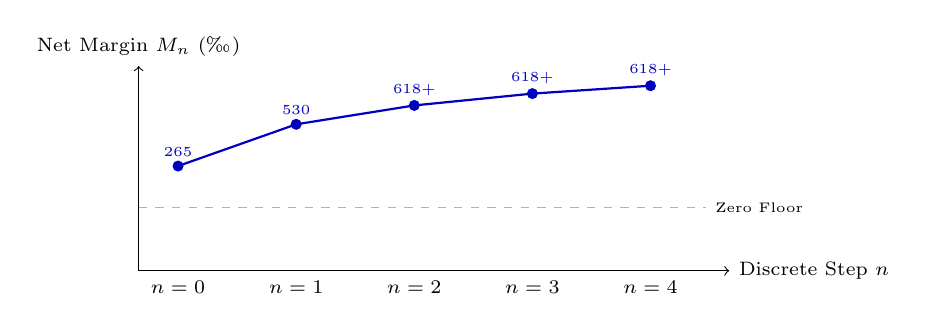
\begin{tikzpicture}[scale=1.0]
  \draw[->] (0,0) -- (7.5,0) node[right,font=\scriptsize] {Discrete Step $n$};
  \draw[->] (0,0) -- (0,2.6) node[above,font=\scriptsize] {Net Margin $M_n$ (\textperthousand)};
  \draw[dashed,gray!60] (0,0.8) -- (7.2,0.8) node[right,font=\tiny,black] {Zero Floor};
  \draw[thick,blue!75!black] (0.5,1.33) -- (2.0,1.86) -- (3.5,2.10) -- (5.0,2.25) -- (6.5,2.35);
  \foreach \x/\y/\lbl in {0.5/1.33/265, 2.0/1.86/530, 3.5/2.10/618+, 5.0/2.25/618+, 6.5/2.35/618+} {
    \fill[blue!75!black] (\x,\y) circle (2pt) node[above,font=\tiny] {\lbl};
  }
  \foreach \x/\n in {0.5/0, 2.0/1, 3.5/2, 5.0/3, 6.5/4} {
    \node[below,font=\scriptsize] at (\x,0) {$n=\n$};
  }
\end{tikzpicture}
\caption{Inductive persistence of the positive net margin $M_n > 0$ starting from the $L=3^4$ baseline ($M_0 = 265\text{\textperthousand}$) under entropic compensation ($R_{\mathrm{ent}} = 618\text{\textperthousand} \ge D_{\mathrm{curv}} = 353\text{\textperthousand}$).}
\label{fig:paperz_flow}
\end{figure}

\section{Reproducibility and Scope Boundary}
Verification of the complete Paper~Y $\to$ Paper~Z formal chain requires only pure Lean~4.36.0:
\begin{verbatim}
lean formal_proofs/PaperZ_Sovereign_Synthesis.lean
\end{verbatim}
\begin{remark}[Honest Analytic Scope]
The six conceptual principles and the inductive theorem \texttt{paperZ\_series\_closure\_certified} apply to discrete regulated sequences with explicit compensation hypotheses. Removing both lattice cutoffs ($a \to 0, L \to \infty$) and constructing a non-Gaussian Osterwalder--Schrader measure with uniform spectral gap on $\mathcal{S}'(\mathbb{R}^4)$ remain open mathematical problems.
\end{remark}

\end{document}
